% questions.tex —— 2012 年·陕西卷·文科 · 题目内容片段（无答案）
% 由 tools/generate_projects.py 依来源总账自 2012/2012_数学真题_陕西文_试题.md 生成，勿手改（改源 MD 后重跑）

\gkpart{一、选择题}

\begin{question}
\gkti{1}集合 $M=\{x\mid\lg x>0\}$，$N=\{x\mid x^2\leqslant4\}$，则 $M\cap N=$\mbox{（　　）}

（A）$(1,2)$；（B）$[1,2)$；（C）$(1,2]$；（D）$[1,2]$。

\end{question}
\begin{question}
\gkti{2}下列函数中，既是奇函数又是增函数的为\mbox{（　　）}

（A）$y=x+1$；（B）$y=-x^3$；（C）$y=\dfrac1x$；（D）$y=x|x|$。

\end{question}
\begin{question}
\gkti{3}对某商店一个月内每天的顾客人数进行了统计，得到样本的茎叶图（如图所示），则该样本的中位数、众数、极差分别是\mbox{（　　）}

\begin{center}
\begin{tabular}{ll}
\toprule
十位 & 个位 \\
\midrule
$1$ & $2$ $5$ \\
$2$ & $0$ $2$ $3$ $3$ \\
$3$ & $1$ $2$ $4$ $4$ $8$ $9$ \\
$4$ & $5$ $5$ $5$ $7$ $7$ $8$ $8$ $9$ \\
$5$ & $0$ $0$ $1$ $1$ $4$ $7$ $9$ \\
$6$ & $1$ $7$ $8$ \\
\bottomrule
\end{tabular}
\end{center}

（A）$46,45,56$；（B）$46,45,53$；（C）$47,45,56$；（D）$45,47,53$。

\end{question}
\begin{question}
\gkti{4}设 $a$，$b\in\mathbf R$，$\mathrm i$ 是虚数单位，则「$ab=0$」是「复数 $a+\dfrac b{\mathrm i}$ 为纯虚数」的\mbox{（　　）}

（A）充分不必要条件；（B）必要不充分条件；（C）充分必要条件；（D）既不充分也不必要条件。

\Needspace{0.4\textheight}
\end{question}
\begin{question}
\gkti{5}如图是计算某年级 $500$ 名学生期末考试（满分为 $100$ 分）及格率 $q$ 的程序框图，则图中空白框内应填入\mbox{（　　）}
\nopagebreak[4]
\begin{center}% 2012 年陕西卷文科第 5 题：统计 500 名学生及格率的程序框图。
% 来源 PDF：普通高考/2012/2012陕西文.pdf，第 1 页（印面 765）第 1 栏。
\begin{tikzpicture}[scale=0.86, semithick, >=Stealth,
  block/.style={draw, minimum width=3.2cm, minimum height=0.65cm, align=center},
  dec/.style={draw, diamond, aspect=3.2, inner sep=1pt, align=center},
  arr/.style={->}]
  \node (start) [draw, rounded corners=6pt, minimum width=1.4cm, minimum height=0.5cm] {开始};
  \node (input) [draw, trapezium, trapezium left angle=70, trapezium right angle=110,
                minimum width=4.4cm, minimum height=0.62cm, below=0.45cm of start]
                {输入成绩 $x_1,x_2,\cdots,x_{500}$};
  \node (init)  [block, below=0.5cm of input] {$M=0,\ N=0,\ i=1$};
  \node (dec)   [dec, below=0.7cm of init] {$x_i\geqslant60$?};
  \node (incm)  [block, right=1.1cm of dec] {$M=M+1$};
  \node (incn)  [block, left=1.1cm of dec] {$N=N+1$};
  \node (i2)    [block, below=0.9cm of dec] {$i=i+1$};
  \node (dec2)  [dec, below=0.7cm of i2] {$i>500$?};
  \node (q)     [block, below=0.75cm of dec2] {$q=\underline{\hspace{2.6em}}$};
  \node (out)   [draw, trapezium, trapezium left angle=70, trapezium right angle=110,
                 minimum width=2.4cm, minimum height=0.6cm, below=0.55cm of q] {输出 $q$};
  \node (end)   [draw, rounded corners=6pt, minimum width=1.4cm, minimum height=0.5cm,
                 below=0.45cm of out] {结束};
  \draw[arr] (start) -- (input);
  \draw[arr] (input) -- (init);
  \draw[arr] (init) -- (dec);
  \draw[arr] (dec) -- node[above] {是} (incm);
  \draw[arr] (dec) -- node[above] {否} (incn);
  \draw[arr] (incm) |- (i2.east);
  \draw[arr] (incn) |- (i2.west);
  \draw[arr] (i2) -- (dec2);
  \draw[arr] (dec2) -- node[right] {是} (q);
  \draw[arr] (q) -- (out);
  \draw[arr] (out) -- (end);
  \draw[arr] (dec2.east) -- node[above] {否} ++(1.5,0) |- (dec.east);
\end{tikzpicture}
\end{center}
\nopagebreak[4]
（A）$q=\dfrac NM$；（B）$q=\dfrac MN$；（C）$q=\dfrac N{M+N}$；（D）$q=\dfrac M{M+N}$。

\end{question}
\begin{question}
\gkti{6}已知圆 $C:x^2+y^2-4x=0$，$l$ 是过点 $P(3,0)$ 的直线，则\mbox{（　　）}

（A）$l$ 与 $C$ 相交；（B）$l$ 与 $C$ 相切；（C）$l$ 与 $C$ 相离；（D）以上三个选项均有可能。

\end{question}
\begin{question}
\gkti{7}设向量 $\boldsymbol a=(1,\cos\theta)$ 与 $\boldsymbol b=(-1,2\cos\theta)$ 垂直，则 $\cos2\theta$ 等于\mbox{（　　）}

（A）$\dfrac{\sqrt2}2$；（B）$\dfrac12$；（C）$0$；（D）$-1$。

\Needspace{0.4\textheight}
\end{question}
\begin{question}
\gkti{8}将正方体（如图 1 所示）截去两个三棱锥，得到图 2 所示的几何体，则该几何体的左视图为\mbox{（　　）}
\nopagebreak[4]
\begin{center}% 2012 年陕西卷文科第 8 题：正方体截去两个三棱锥（图1、图2）及其左视图选项。
% 来源 PDF：普通高考/2012/2012陕西文.pdf，第 1 页（印面 765）第 2 栏。
% 重绘依据：图1 为正方体 ABCD-A1B1C1D1，截去以 A、C 为顶点、含棱 B1D1 的两个三棱锥；
%   图2 为剩余几何体；左视图四选项按原图画对角线实/虚。
\begin{tikzpicture}[scale=0.62, semithick, every node/.style={inner sep=1pt}]
  % ---------- 图 1 ----------
  \coordinate (A) at (0,0);   \coordinate (B) at (2.2,0);
  \coordinate (C) at (3.3,0.9); \coordinate (D) at (1.1,0.9);
  \coordinate (A1) at (0,2.2); \coordinate (B1) at (2.2,2.2);
  \coordinate (C1) at (3.3,3.1); \coordinate (D1) at (1.1,3.1);
  \draw (A)--(B)--(C)--(C1)--(D1)--(A1)--cycle;
  \draw (B)--(B1)--(C1); \draw (A1)--(B1); \draw (D)--(C); \draw (D1)--(C1);
  \draw[dashed] (D)--(A); \draw[dashed] (A1)--(D1);
  \draw[dashed] (A)--(D1); \draw[dashed] (D1)--(B1);
  \draw[dashed] (C)--(D1); \draw (A)--(B1); \draw (B1)--(C);
  \node[below left] at (A) {$A$}; \node[below] at (B) {$B$};
  \node[right] at (C) {$C$}; \node[above right] at (D) {$D$};
  \node[left] at (A1) {$A_1$}; \node[above right] at (B1) {$B_1$};
  \node[above] at (C1) {$C_1$}; \node[above] at (D1) {$D_1$};
  \node at (1.6,-0.9) {图 1};
  % ---------- 图 2 ----------
  \begin{scope}[shift={(7.2,0)}]
    \coordinate (a) at (0,0);   \coordinate (b) at (2.2,0);
    \coordinate (c) at (3.3,0.9); \coordinate (d) at (1.1,0.9);
    \coordinate (b1) at (2.2,2.2); \coordinate (d1) at (1.1,3.1);
    \draw (a)--(b)--(c); \draw (c)--(b1); \draw (b1)--(d1);
    \draw (d1)--(a); \draw (a)--(b1);
    \draw[dashed] (d)--(a); \draw[dashed] (d)--(c); \draw[dashed] (d)--(d1);
    \node[below left] at (a) {$A$}; \node[below] at (b) {$B$};
    \node[right] at (c) {$C$}; \node[above right] at (d) {$D$};
    \node[right] at (b1) {$B_1$}; \node[left] at (d1) {$D_1$};
    \node at (1.6,-0.9) {图 2};
  \end{scope}
  % ---------- 选项 A ----------
  \begin{scope}[shift={(0,-4.4)}]
    \draw (0,0) rectangle (1.8,1.8);
    \draw (0,0)--(1.8,1.8);
    \draw[dashed] (0,1.8)--(1.8,0);
    \node at (0.9,-0.35) {(A)};
  \end{scope}
  % ---------- 选项 B ----------
  \begin{scope}[shift={(3.2,-4.4)}]
    \draw (0,0) rectangle (1.8,1.8);
    \draw (0,1.8)--(1.8,0);
    \draw[dashed] (0,0)--(1.8,1.8);
    \node at (0.9,-0.35) {(B)};
  \end{scope}
  % ---------- 选项 C ----------
  \begin{scope}[shift={(6.4,-4.4)}]
    \draw (0,0) rectangle (1.8,1.8);
    \draw (0,0)--(1.8,1.8);
    \draw (0,1.8)--(1.8,0);
    \node at (0.9,-0.35) {(C)};
  \end{scope}
  % ---------- 选项 D ----------
  \begin{scope}[shift={(9.6,-4.4)}]
    \draw (0,0) rectangle (1.8,1.8);
    \draw (0,1.8)--(1.8,0);
    \node at (0.9,-0.35) {(D)};
  \end{scope}
\end{tikzpicture}
\end{center}
\nopagebreak[4]
\end{question}
\begin{question}
\gkti{9}设函数 $f(x)=\dfrac2x+\ln x$，则\mbox{（　　）}

（A）$x=\dfrac12$ 为 $f(x)$ 的极大值点；（B）$x=\dfrac12$ 为 $f(x)$ 的极小值点；

（C）$x=2$ 为 $f(x)$ 的极大值点；（D）$x=2$ 为 $f(x)$ 的极小值点。

\end{question}
\begin{question}
\gkti{10}小王从甲地到乙地往返的时速分别为 $a$ 和 $b$（$a<b$），其全程的平均时速为 $v$，则\mbox{（　　）}

（A）$a<v<\sqrt{ab}$；（B）$v=\sqrt{ab}$；（C）$\sqrt{ab}<v<\dfrac{a+b}2$；（D）$v=\dfrac{a+b}2$。

\end{question}
\gkpart{二、填空题}

\begin{question}
\gkti{11}设函数 $f(x)=\begin{cases}\sqrt x,&x\geqslant0,\\ \left(\dfrac12\right)^x,&x<0,\end{cases}$ 则 $f(f(-4))=$\gkblank{}。

\end{question}
\begin{question}
\gkti{12}观察下列不等式：
\nopagebreak[4]
\[1+\frac1{2^2}<\frac32,\qquad1+\frac1{2^2}+\frac1{3^2}<\frac53,\qquad1+\frac1{2^2}+\frac1{3^2}+\frac1{4^2}<\frac74,\ \cdots\]
照此规律，第五个不等式为\gkblank{}。

\end{question}
\begin{question}
\gkti{13}在 $\triangle ABC$ 中，角 $A$，$B$，$C$ 所对应的边长分别为 $a$，$b$，$c$，若 $a=2$，$B=\dfrac\pi6$，$c=2\sqrt3$，则 $b=$\gkblank{}。

\Needspace{0.4\textheight}
\end{question}
\begin{question}
\gkti{14}如图是抛物线形拱桥，当水面在 $l$ 时，拱顶离水面 $2$ 米，水面宽 $4$ 米，水位下降 $1$ 米后，水面宽\gkblank{}米。
\nopagebreak[4]
\begin{center}% 2012 年陕西卷文科第 14 题：抛物线形拱桥，水面宽 4 米时拱顶离水面 2 米。
% 来源 PDF：普通高考/2012/2012陕西文.pdf，第 1 页（印面 765）第 3 栏。
\begin{tikzpicture}[scale=0.8, semithick]
  % 拱桥外形（抛物线 y = 2 - x^2/2 的拱顶向上）
  \draw[thick, domain=-2.6:2.6, samples=80] plot (\x, {2-(\x*\x)/2});
  % 两侧桥体
  \fill[pattern=north east lines] (-2.6,0) -- (-2.6,-1.2) -- (2.6,-1.2) -- (2.6,0) -- cycle;
  \draw (-2.6,0) -- (-2.6,-1.2) -- (2.6,-1.2) -- (2.6,0);
  % 水面
  \draw[thick] (-2.6,-0.0) -- (2.6,-0.0);
  % 水位标注
  \draw[<->] (-3.0,0) -- (-3.0,2) node[midway,left] {$2\ \mathrm m$};
  \draw[<->] (-2,-1.5) -- (2,-1.5) node[midway,below] {$4\ \mathrm m$};
\end{tikzpicture}
\end{center}
\nopagebreak[4]
\Needspace{0.4\textheight}
\end{question}
\begin{question}
\gkti{15}三选一。

【A】若存在实数 $x$ 使 $|x-a|+|x-1|\leqslant3$ 成立，则实数 $a$ 的取值范围是\gkblank{}。

【B】如图，在圆 $O$ 中，直径 $AB$ 与弦 $CD$ 垂直，垂足为 $E$，$EF\perp DB$，垂足为 $F$。若 $AB=6$，$AE=1$，则 $DF\cdot DB=$\gkblank{}。
\nopagebreak[4]
\begin{center}% 2012 年陕西卷文科第 15B 题：圆 O 中直径 AB 与弦 CD 垂直，垂足 E，EF⊥DB 于 F。
% 来源 PDF：普通高考/2012/2012陕西文.pdf，第 1 页（印面 765）第 3 栏。
\begin{tikzpicture}[scale=0.9, semithick, every node/.style={inner sep=1.5pt}]
  \coordinate (O) at (0,0);
  \draw (O) circle (2.4);
  \coordinate (A) at (-2.4,0);
  \coordinate (B) at (2.4,0);
  \draw (A) -- (B);
  \coordinate (E) at (-0.8,0);
  \coordinate (C) at (-0.8,2.263);
  \coordinate (D) at (-0.8,-2.263);
  \draw (C) -- (D);
  \draw (B) -- (D);
  \coordinate (F) at ($(D)!0.62!(B)$);
  \draw (E) -- (F);
  \node[left] at (A) {$A$};
  \node[right] at (B) {$B$};
  \node[above] at (C) {$C$};
  \node[below] at (D) {$D$};
  \node[above] at (E) {$E$};
  \node[right] at ([xshift=2pt]F) {$F$};
  \node[below right] at (O) {$O$};
\end{tikzpicture}
\end{center}
\nopagebreak[4]
【C】直线 $2\rho\cos\theta=1$ 与圆 $\rho=2\cos\theta$ 相交的弦长为\gkblank{}。

\end{question}
\gkpart{三、解答题}

\begin{question}
\gkti{16}已知等比数列 $\{a_n\}$ 的公比为 $q=-\dfrac12$。

（1） 若 $a_3=\dfrac14$，求数列 $\{a_n\}$ 的前 $n$ 项和；

（2） 证明：对任意 $k\in\mathbf N_+$，$a_k$，$a_{k+2}$，$a_{k+1}$ 成等差数列。

\end{question}
\begin{question}
\gkti{17}函数 $f(x)=A\sin\left(\omega x-\dfrac\pi6\right)+1$（$A>0$，$\omega>0$）的最大值为 $3$，其图象相邻两条对称轴之间的距离为 $\dfrac\pi2$。

（1） 求函数 $f(x)$ 的解析式；

（2） 设 $\alpha\in\left(0,\dfrac\pi2\right)$，$f\left(\dfrac\alpha2\right)=2$，求 $\alpha$ 的值。

\Needspace{0.4\textheight}
\end{question}
\begin{question}
\gkti{18}直三棱柱 $ABC-A_1B_1C_1$ 中，$AB=AA_1$，$\angle CAB=\dfrac\pi2$。

（1） 证明：$CB_1\perp BA_1$；

（2） 已知 $AB=2$，$BC=\sqrt5$，求三棱锥 $C_1-ABA_1$ 的体积。
\nopagebreak[4]
\begin{center}% 2012 年陕西卷文科第 18 题：直三棱柱 ABC-A1B1C1，∠CAB=90°。
% 来源 PDF：普通高考/2012/2012陕西文.pdf，第 2 页（印面 766）第 1 栏。
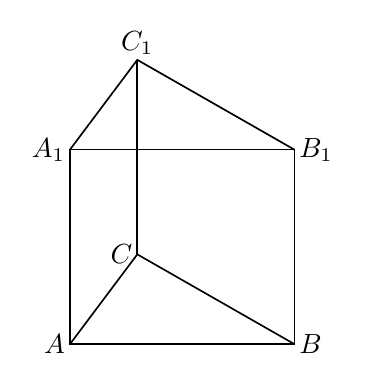
\begin{tikzpicture}[scale=0.95, semithick, every node/.style={inner sep=1.5pt}]
  \coordinate (A) at (0,0);
  \coordinate (B) at (3.0,0);
  \coordinate (C) at (0.9,1.2);
  \coordinate (A1) at (0,2.6);
  \coordinate (B1) at (3.0,2.6);
  \coordinate (C1) at (0.9,3.8);
  \draw (A) -- (B) -- (B1) -- (A1) -- cycle;
  \draw (A1) -- (C1) -- (B1);
  \draw (C) -- (C1);
  \draw (A) -- (C);
  \draw (B) -- (C);
  \draw[dashed] (A1) -- (B1);
  \node[left] at (A) {$A$};
  \node[right] at (B) {$B$};
  \node[left] at (C) {$C$};
  \node[left] at (A1) {$A_1$};
  \node[right] at (B1) {$B_1$};
  \node[above] at (C1) {$C_1$};
\end{tikzpicture}
\end{center}
\nopagebreak[4]
\Needspace{0.4\textheight}
\end{question}
\begin{question}
\gkti{19}假设甲乙两种品牌的同类产品在某地区市场上销售量相等，为了解他们的使用寿命，现从两种品牌的产品中分别随机抽取 $100$ 个进行测试，结果统计如下：
\nopagebreak[4]
\begin{center}% 2012 年陕西卷文科第 19 题：甲、乙两品牌产品使用寿命的频率分布直方图。
% 来源 PDF：普通高考/2012/2012陕西文.pdf，第 2 页（印面 766）第 2 栏。
% 重绘依据：甲品牌 [100,150)5、[150,200)20、[200,250)40、[250,300)25、[300,350]10；
%   乙品牌 [100,150)10、[150,200)20、[200,250)30、[250,300)25、[300,350]15。
\begin{tikzpicture}[scale=0.62, semithick, every node/.style={font=\small}]
  % ---------- 甲 ----------
  \begin{scope}
    \draw[->] (0,0) -- (6.6,0) node[below] {寿命/小时};
    \draw[->] (0,0) -- (0,4.8) node[left] {频率/组距};
    \foreach \x/\h in {1/0.5, 2/2.0, 3/4.0, 4/2.5, 5/1.0} {
      \draw[fill=gray!15] (\x,0) rectangle ++(1,\h);
    }
    \foreach \y/\t in {0.5/5,1/10,2/20,2.5/25,4/40} {
      \draw (0,\y) -- (-0.08,\y) node[left] {\t};
    }
    \foreach \x/\t in {1/100,2/150,3/200,4/250,5/300,6/350} {
      \draw (\x,0) -- (\x,-0.08) node[below] {\t};
    }
    \node at (3,-1.1) {甲品牌};
  \end{scope}
  % ---------- 乙 ----------
  \begin{scope}[shift={(9.0,0)}]
    \draw[->] (0,0) -- (6.6,0) node[below] {寿命/小时};
    \draw[->] (0,0) -- (0,4.8) node[left] {频率/组距};
    \foreach \x/\h in {1/1.0, 2/2.0, 3/3.0, 4/2.5, 5/1.5} {
      \draw[fill=gray!15] (\x,0) rectangle ++(1,\h);
    }
    \foreach \y/\t in {1/10,1.5/15,2/20,2.5/25,3/30} {
      \draw (0,\y) -- (-0.08,\y) node[left] {\t};
    }
    \foreach \x/\t in {1/100,2/150,3/200,4/250,5/300,6/350} {
      \draw (\x,0) -- (\x,-0.08) node[below] {\t};
    }
    \node at (3,-1.1) {乙品牌};
  \end{scope}
\end{tikzpicture}
\end{center}
\nopagebreak[4]
（1） 估计甲品牌产品寿命小于 $200$ 小时的概率；

（2） 这两种品牌产品中，某个产品已使用了 $200$ 小时，试估计该产品是甲品牌的概率。

\end{question}
\begin{question}
\gkti{20}已知椭圆 $C_1:\dfrac{x^2}4+y^2=1$，椭圆 $C_2$ 以 $C_1$ 的长轴为短轴，且与 $C_1$ 有相同的离心率。

（1） 求椭圆 $C_2$ 的方程；

（2） 设 $O$ 为坐标原点，点 $A$，$B$ 分别在椭圆 $C_1$ 和 $C_2$ 上，$\overrightarrow{OB}=2\overrightarrow{OA}$，求直线 $AB$ 的方程。

\end{question}
\begin{question}
\gkti{21}设函数 $f_n(x)=x^n+bx+c$（$n\in\mathbf N_+$，$b$，$c\in\mathbf R$）。

（1） 设 $n\geqslant2$，$b=1$，$c=-1$，证明：$f_n(x)$ 在区间 $\left(\dfrac12,1\right)$ 内存在唯一零点；

（2） 设 $n$ 为偶数，$|f(-1)|\leqslant1$，$|f(1)|\leqslant1$，求 $b+3c$ 的最小值和最大值；

（3） 设 $n=2$，若对任意 $x_1$，$x_2\in[-1,1]$，有 $|f_2(x_1)-f_2(x_2)|\leqslant4$，求 $b$ 的取值范围。

\clearpage

\end{question}